\documentclass[12pt, a4paper]{article}
\usepackage[margin=0.5in]{geometry}

\usepackage{color}
\usepackage[dvipsnames]{xcolor}
\usepackage{hyperref}
\hypersetup{
    colorlinks=true,
    linkcolor=blue,
    urlcolor=blue,
    linktoc=all
}


\usepackage{amsmath}
\usepackage{mathtools}
\usepackage{amssymb}
\usepackage{cancel}
\usepackage{bm}
\usepackage{dsfont}
\usepackage{graphicx}
\usepackage{graphics}
\usepackage{xfrac}
\usepackage{array}
\setcounter{MaxMatrixCols}{40}

\usepackage{enumerate}
\usepackage{enumitem}
\usepackage{multirow}

%inclusions carried over from past class homework formats
\usepackage{units}
\usepackage{fullpage}
\usepackage{alltt}
\usepackage{mathrsfs}
\usepackage{xcolor}
\usepackage{soul}

\usepackage{pgfplots}

\DeclarePairedDelimiter{\abs}{\lvert}{\rvert}
\newcommand*{\fontCourier}{\fontfamily{pcr}\selectfont}
\newcommand*\mean[1]{\overline{#1}}
\newcommand\scalemath[2]{\scalebox{#1}{\mbox{\ensuremath{\displaystyle #2}}}}

\setcounter{tocdepth}{5}
\setcounter{secnumdepth}{5}

% \usepackage{pdfpages}
\usepackage{Sweave}
\begin{document}
% 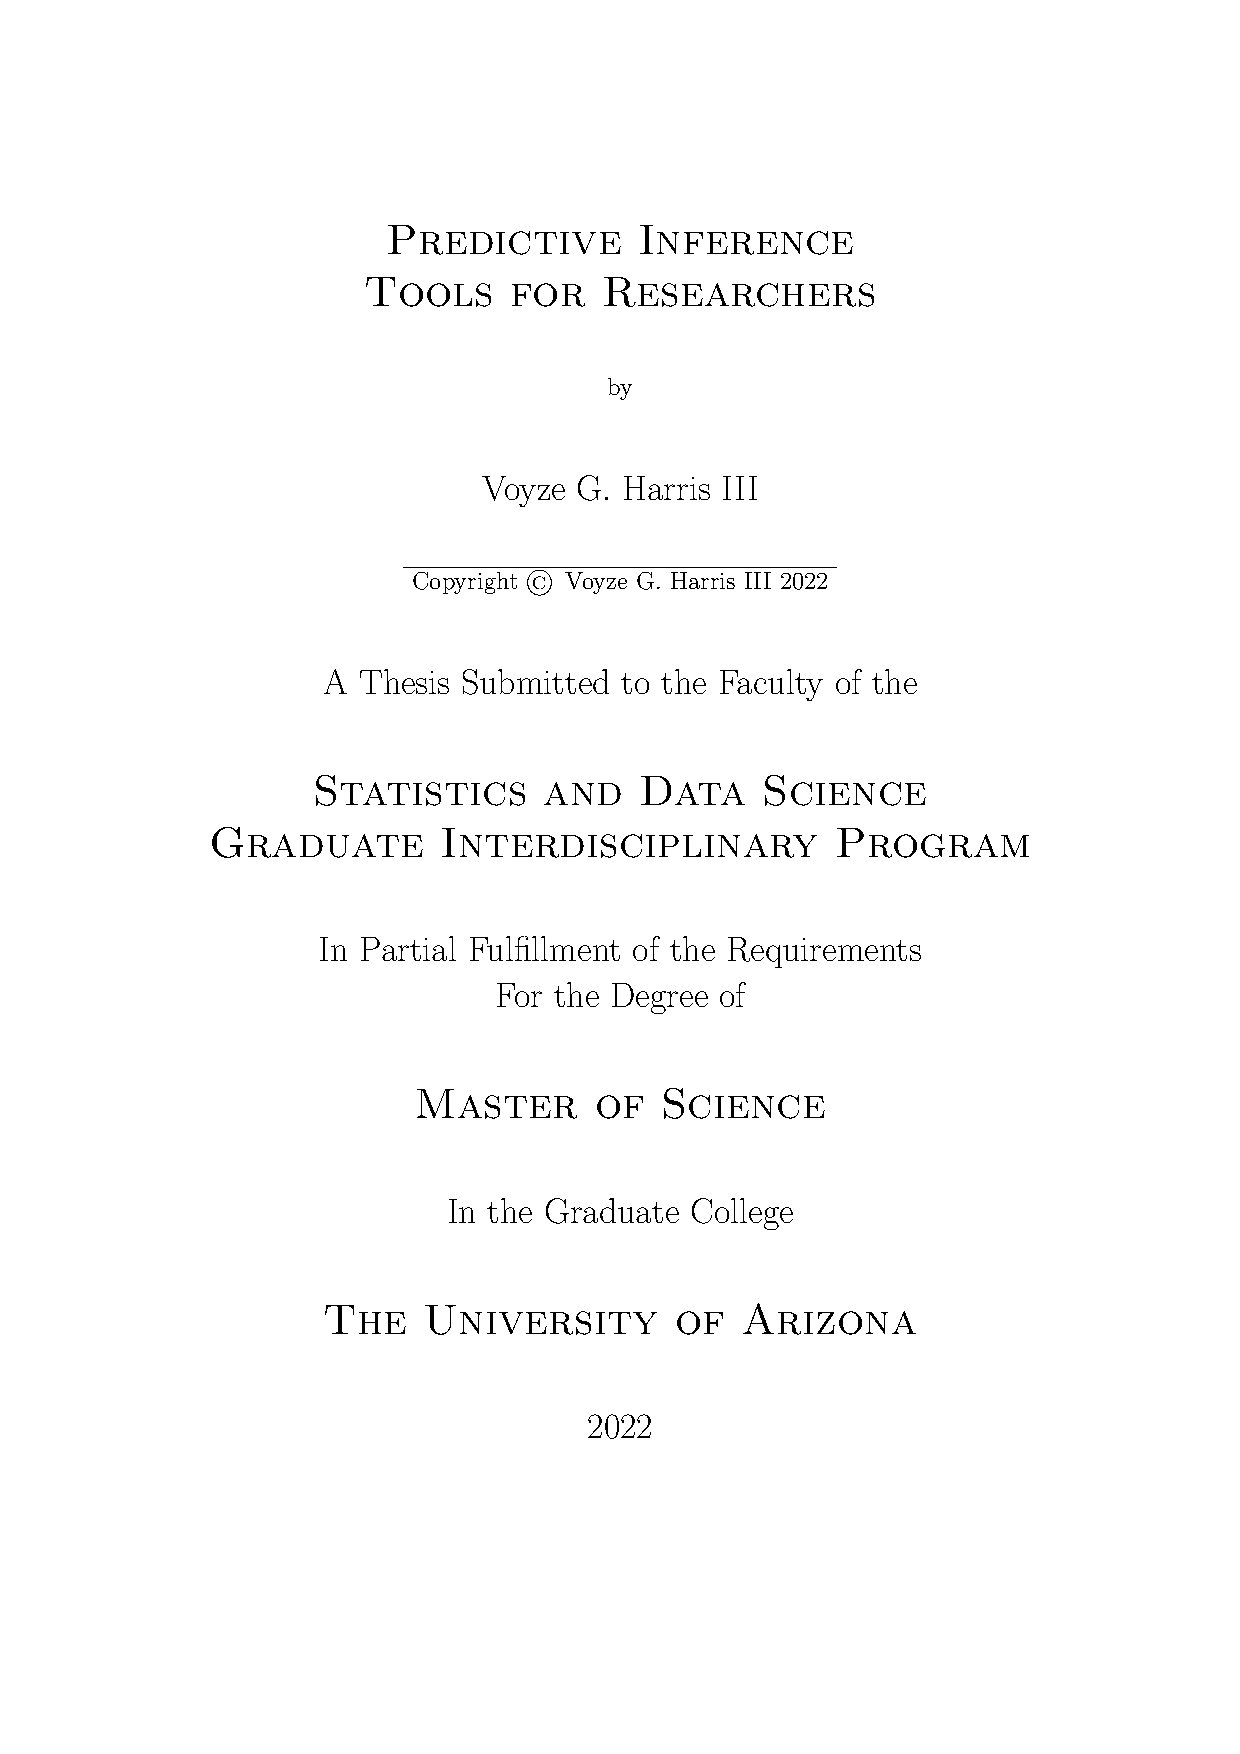
\includepdf{TitlePage_MastersThesis}
% 
\includepdf{ThesisApprovalPage}
\Sconcordance{concordance:DeanArticleNotes.tex:DeanArticleNotes.Rnw:%
1 49 1 1 0 7 1 1 4 66 1}


% \tableofcontents
% \newpage



\title{Notes on ``Predictive Inference and Scientific Reproducibility" by Dean Billheimer}
\author{\Large Gabe Harris}
\maketitle

\textbf{Abstract}\\
\begin{itemize}
  \item hypothesis tests and parameter estimation for inference are ``noble, but misguided."
  \item "observables are fundamental"
  \item prediction of future observables given current data and understanding is the goal of statistical modeling
  \item Advantages of predicting future observables:
    \begin{itemize}
      \item ``an interpretable numerical summary of a quantity of direct interest to current and future researchers"
      \item ``a calibrated prediction of what's likely to happen in future experiments"
      \item ``a prediction that can be either `corroborated' or `refuted' through experimentation"
      \item ``avoidance of inference about parameters; quantities that exist only as convenient indices of hypothetical distributions"
    \end{itemize}
  \item ``Adoption of this paradigm would improve our rigor for scientific accuracy and reproducibility by shifting our focus from `finding differences' among hypothetical parameters to predicting observable events based on our current scientific understanding."
  \item \textcolor{red}{Elaborate on how prediction improves ``rigor for scientific accuracy and reproducibility"?  Concrete examples?}
\end{itemize}

\textit{``The only useful function for a statistician is to make predictions, and thus provide a basis for action."}\\
W. Edwards Deming\\

\section{Introduction}

\begin{itemize}
  \item ``current disciplinary dilemma over $p$-values," conventional hypothesis tests.  Conventional ways of doing statistics compromises reproducibility \textcolor{red}{elaborate}
  \item misguided to try to ``fix" hypothesis testing
  \item ``larger and deeper inferential problems"
    \begin{itemize}
      \item ``dichotomization of results as either `significant' or `nonsignificant'"
      \item ``the failure to incorporate the consequences of different types of testing errors"
      \item ``unclear definition of what it means to `reproduce' a result"
    \end{itemize}
  \item scientists without expertise in statistics are frustrated with follow-on experiments that do not provide `significant' results, despite indications from traditional hypothesis testing and confidence intervals.  This is a failure of statistics.
  \item ``A focus on prediction allows the comparison of competing theories according to the quality of predictions they make, thus leading to better scientific inference."
  \item reliability and validity in educational and psychometric testing theory
    \begin{itemize}
      \item reliability:  stability of measurement
      \item validity:  meaningfulness of the measurement
      \item ``Probabilistic prediction ... constitutes a type of `measurement reliability'  for inferences"
      \item ``focus on observable events, rather than unobservable parameters, ensures the `meaningfulness' of results for future investigators"
    \end{itemize}
\end{itemize}

Additional advantages
\begin{itemize}
  \item focus on important (to the study) quantities, avoiding less informative inferential summaries ``that arise historically because of their convenient sampling properties"
  \item ``interpretation of `causes'" (e.g. regression parameter estimates) ``based on the entire distribution of observables, thus encouraging the identification of relevant changes" \textcolor{red}{elaborate}
  \item ``the practical significance conferred to individuals...avoiding paradoxes of practical vs. statistical significance."  \textcolor{red}{elaborate?  examples?}
  \item interpretation of experimental results as sequential and progressive, with later results related to and influenced by earlier ones $\rightarrow$ better reproducibility \textcolor{red}{so I'm thinking reproducibility is enhanced progressively through the process of iterated experiments with updated prior information}
  \item ``full accounting of the variability contributing to, or inherent in, the observed data, avoiding uncertainty laundering (Gelman 2016)" \textcolor{red}{What is ``uncertainty laundering"?}
\end{itemize}

More fundamental advantage:  ``predictions of observable events is understandable to humans."









\end{document}
